\documentclass[11pt,a5paper,oneside]{book}

\usepackage[
	top=1cm,
	bottom=1cm,
	left=1.5cm,
	right=2.5cm,
	headheight=17pt,
	includehead,includefoot,
	heightrounded,
]{geometry}

\usepackage[finnish]{babel}
\usepackage[utf8]{inputenc}
\usepackage[T1]{fontenc}

\title{Pion. P 32:n sotapäiväkirja (19826)}
% http://digi.narc.fi/digi/slistaus.ka?ay=80360

\usepackage{longtable}
\usepackage{setspace}
\usepackage{romannum}
\usepackage{graphicx}
\usepackage{ulem}
\usepackage{siunitx}
\usepackage{xfrac}
\usepackage{fix-cm}

\usepackage{hyperref}
\hypersetup{
    colorlinks=true,
    linkcolor=blue,
    filecolor=magenta,      
    urlcolor=blue,
}
\urlstyle{same}

\usepackage{xcolor}

\usepackage{changepage}
\usepackage{fancyhdr}
\usepackage{extramarks}
\pagestyle{fancy}
\fancypagestyle{headings}

%% L/C/R denote left/center/right header (or footer) elements
%% E/O denote even/odd pages

%% \leftmark, \rightmark are chapter/section headings generated by the 
%% book document class

%\fancyhead[C]{}
%\fancyhead[C]{\slshape Pion. P 32:n sotapäiväkirja}
\fancyhead[L]{}
\fancyhead[C]{Pion. P 32:n sotapäiväkirja 1941-1941 (19826)}
\fancyhead[R]{\firstxmark}
\fancyfoot[]{}
%\fancyhead[R]{\thepage}

\begin{document}
\pagenumbering{arabic}

\extramarks{}{}

\begin{titlepage}
	\begin{center}
		\vspace*{1.5cm}
        \href{http://digi.narc.fi/digi/view.ka?kuid=3753911}{\Large Tulo 1264} \\
       	\vspace{1.5cm}
        \textbf{\Large Pion. P 32} \\
       	\vspace{1.5cm}
		\textbf{\Huge SOTAPÄIVÄKIRJA} \\
		\vspace{1.5cm}
		\Large 16.6.1941-17.10.1941 \\
   	\end{center}
\end{titlepage}

\extramarks{}{}
\section*{Esipuhe}
\setcounter{page}{2}
Tämä sotapäiväkirja perustuu Kansallisarkiston digitaaliarkistosta löytyviin digitoituihin jaksoihin arkistoyksiköstä Pioneeripataljoona 32 1941-1941 (19826), joka löytyy osoitteesta: \\
\url{http://digi.narc.fi/digi/slistaus.ka?ay=80360} \\

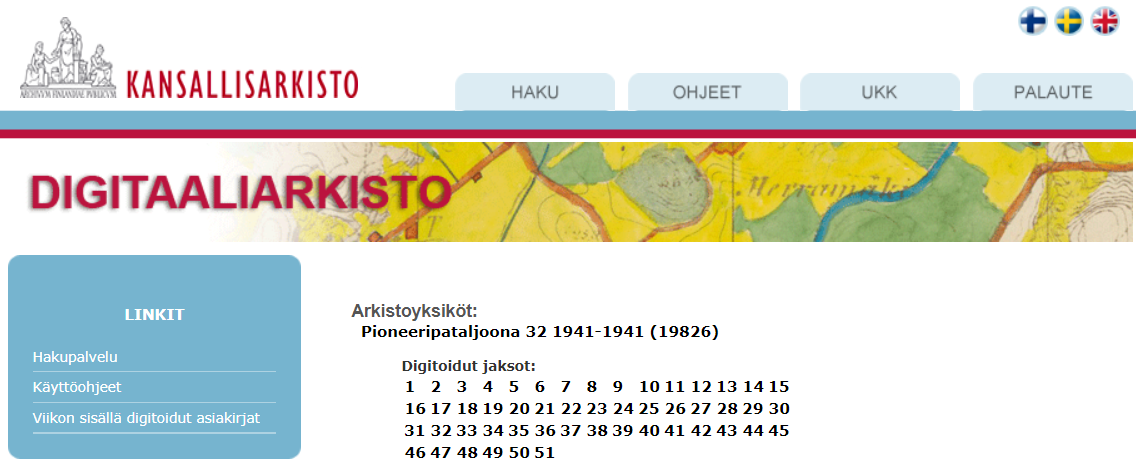
\includegraphics[scale=0.45]{jaksot_19826.png}

Kunkin sivun ylätunnisteessa oikeall on kyseisen digitoidun jakson numero ja linkki siihen kansallisarkiston digitoituun jaksoon.

Mikäli sotapäiväkirjan digitoidusta jaksossa on ollut vaikeuksia sanojen/merkintöjen tulkinnassa niin ne kohdat on merkitty \textcolor{red}{punaisella}. Linkki alkuperäiseen digitoituun jaksoon auttaa selvittämään näiden merkintöjen oikean merkityksen.

Sitä mukaa kun tekstissä on tullut lyhenteitä tai sanoja, joita lukija ei välttämättä tiedä niin näitä on pyritty selventämään sivun alalaidassa olevilla alaviitteillä. Lisäksi jokainen paikannimi on mainittu alaviitteissä helpottaakseen lukijaa seuraamaan etenemistä kartalta. Alaviitteissä saattaa löytyä myös muuta asiaan liittyvää lisäinformaatiota. Näitä alaviitteitä ei ole alkuperäisessä sotapäiväkirjassa.
%\FloatBarrier

\newcommand{\taulustart}[2]{
\newpage\extramarks{\href{#1}{#2}}{}
\begin{center} % optimoitu A5 formaattiin:
\renewcommand*{\arraystretch}{1.4}
\begin{longtable}{ | p{0.14\textwidth} | p{0.09\textwidth} | p{0.77\textwidth} |}
\hline \multicolumn{1}{|p{0.14\textwidth}|}{\textbf{Päiväys}} & \multicolumn{1}{p{0.09\textwidth}|}{\textbf{Kello}} & \multicolumn{1}{p{0.77\textwidth}|}{\textbf{SISÄLTÖ}} \\ \hline
\endfirsthead
\hline \multicolumn{1}{|p{0.14\textwidth}|}{\textbf{Päiväys}} & \multicolumn{1}{p{0.09\textwidth}|}{\textbf{Kello}} & \multicolumn{1}{p{0.77\textwidth}|}{\textbf{SISÄLTÖ}} \\ \hline
\endhead \hline \endfoot \hline \endlastfoot}

\newcommand{\taulustop}{\hline \end{longtable} \end{center} \newpage}
\taulustart{http://digi.narc.fi/digi/view.ka?kuid=3753912}{2}

16.6.41 & 11.00 & Kokoontuminen Lohjan Kauppalan Yhteiskoululla\footnote{\href{https://www.google.fi/maps/place/Suurlohjankatu+2,+08100+Lohja/}{Lohjan yhteiskoulu 1915-1957, Suurlohjankatu 2, Lohja}}. Perustamispaikka ei ollut sopiva. Kun pataljoonan muodostavat reserviläiset olivat etupäässä lohjalaisia oli järjestyksen ylläpitäminen vaikeanlainen. Lisäksi vaikeutti perustamistapaikaksi valittu Yhteiskoulun pienuus järjestyksen ylläpitämistä. \\
% Lohjan Kauppalan Yhteiskoulu toimi aluksi vuokralla Anttilan talon vanhassa asuinrakennuksessa osoitteessa Suurlohjankatu 2, Lohja.

17.6.41 & 19.30 & Lähtivät kapt. Marrasmaa, luutn. Raimoranta, vänr. Helanto ja \textcolor{red}{ajomies} henkilöautolla Grabbskog träskiin\footnote{\href{https://www.google.fi/maps/place/Stortr\%C3\%A4sket/@60.0191777,23.3441542,15z}{Grabbskog Storträsket, Raasepori}} käskyn mukaisella tiedustelumatkalla yhteysottoon HR\footnote{Hangon Ryhmä}:ään.\\
% Träsk on ruotsia ja se on suomeksi järvi. Kartasta löytyy Grabbskog Storträsket Raaseporin läheisyydestä.

17.6.41 & 11.00 & Yksikköjen tuntolevyluettelot, ylimääräiset A- ja lääk. kortit lähetettiin SA-käskun mukaan Lohjan sk. toimistoon. Samoin luettelot puuttuvista korteista. 3 komppannian jako suoritettiin loppuun. Edelleen määrättiin lopullisesti kunkin yksikön päälliköt ja esikunnan kokoon- \\
\newpage

& & pano: Patalj. kom. Kapt. Marrasmaa,\newline adj. luutn. A. Gustafsson \newline pion. ups. luutn. I. Laatinen\newline talousups. luutn. S. Kärki \newline Autoups. luutn. J. Brax \newline 1.K.pääll. Ins. Kapt. Hotinen \newline 2.K.pääll. luutn. Korhonen \newline 3.K.pääll. luutn. Raimoranta \newline Valonheitinj. johtajaksi määrättiin vääpeli Huhtanen. \newline Raimorannan kompp. muodosti 13. Prikaatin pion. Komppaniat.\\

& 12.00 & Alkoi keskitysmarssi. Autorivistö lähti 12.07, johon kuului Esik., Valonheitinj. ja 2 K. johtajana luutn. Laatinen. \\

& 15.00 & Esik. ja 2 K-/ auto saapui Grabbskogträskiin. \\

& 16.15 & Lähetettiin 5 km auton hakemaan 1 K:aa \\

19.6.41 & 2.00 & Saapui 1 K:n miehet Leksvalliin\footnote{\href{https://www.google.fi/maps/place/10660+Leksvall/}{Leksvall, Raasepori}}. \\

& 7.30 & Hevoset saapuvat Grabbskogträskiin. \\

& 7.45 & Ensimmäinen valm. ilmoitus. \newline $a=\frac{137}{19}$, $b=\frac{84}{82}$, $e=\frac{92}{424}$, $d=\frac{92}{532}$ \\
\taulustop

\taulustart{http://digi.narc.fi/digi/view.ka?kuid=3753913}{3}

19.6. & 9.15 & 3 Komppanian au-jaettiin, 5 au 1 K:aan ja 3 2:aan. \\

19.6-20.6 & & Majoitusjärjestelyjä. Ei mitään erikoista. 1 H-auto, 1 \textcolor{red}{ku}-auto ja 1 mp lisää Lohjalta. Esikunnan joukot epäkunnossa. Korjattu iltaan mennessä. 1 K:n pääll. Kapteeni Hotinen siirrettiin HR:n \textcolor{red}{Tukikohtaan}. Samoin vänr. \textcolor{red}{Ilomin} ja Koivula. Edellämainittu Pion. toimistoon. \newline 1 Kompp. ollut miinoitustyössä \newline 2 Kompp. järjestynyt majoitukseen ja osa ollut tietyössä\\ 

21.6. & 7.00 & Vaun. maitoa \newline Kävin DE:ssä, Maj. Laakso antoi määräyksen ruuhikaluston\footnote{\url{https://elavamuisti.fi/aikajana/ruuhikaluston-kaytto}} kuntoon laittamisesta. En vieläkään saanut karttoja. Meidän on itse koulutettava erikoismiehistömme. Osa Pion. kalustosta siirrettiin Pion. Tp:hen. \underline{\textcolor{red}{Kanttiini}} valmistui. 11 miestä siirrettiin 3 K:sta 2 K:hon.\\

22.6. & 7.00 & valm. ilm. $a=137, b=87, e=102, d=100$ \\
\newpage
& 7.00 & Ilmoitukset \%:ssa kokovahvuudesta = 100\%, autovahvuus 31 \%, hevosvahvuus 100 \%.\\ 

& 16.10 & \underline{Pion. Kom. kirje 31}/Pion./\Romannum{2}/F/sal. Kompp. \newline Koulutuksesta: 11. ja 2 K noudatettava yleistä kertausharjoituskoulutusohjeita. 3 K:n koulutuksen painopiste tulee olla rynnäkköpion. koulutuksessa siten, että \textcolor{red}{u} joukkue pystyy väkivaltaiseen ylimenoon.\newline Pataljoonan on suoritettava tiedustelua mahdollista ylimenoa varten peitepiirroksessa mainitulla linjalla 1/A-B ja ryhdyttävä valmistamaan uivaa siltaa kohdassa L (Solböle\footnote{\href{https://www.google.fi/maps/place/10570+Solb\%C3\%B6le/}{Solböle, Raasepori}}) \newline Kirje 32/Tietetio/\Romannum{3}/sal. mukaan on patalj. ryhdyttävä tientekoon alkaen A:sta ja huomioimattaan sen, ettei muu pion. koulutus kärsi. Tie tehtävä yhteen suuntaan liikennöitäväksi autotieksi \textcolor{red}{sivuuten kohteisiin.} \\

23.6. & & Yhteys JR 55:en everstil. Wiberg. Keskusteltiin tien A-B rakentamisesta. Pyydettiin apua. Ei tule? \\

\taulustop

\taulustart{http://digi.narc.fi/digi/view.ka?kuid=3753914}{4}

23.6. & & Ilmoitettu komppanioille hälytysvalmiudesta. Vänr. \textcolor{red}{Sjöblom} 2 au pat. Haartmanin käyttöön. \\

& 18.00 & valm. ilm. $a=131, b=89, e=103, d=132$ \newline valm. ilm. 1) 102, 2) 49, 3) 100. \\

24.6. & & Valm. ilm. sama kuin ennen\newline 3 K. alistettu muualle.\newline Saatu uusia tehtäviä:\newline 1 K \underline{Miinakenttää} ei saa rakentaa lisää.\newline Radan korjausvälineet otettiin pois Skogbyhyn\footnote{\href{https://www.google.fi/maps/place/10680+Skogby/}{Skogby, Raasepori}} saakka. Skogby-järven ympäri tehtiin tie. Lehvallin laiturin viimeistely. Rautatien \textcolor{red}{poly} puolella oleva rataylimenopaikat valmistetaan.\newline \underline{Oikotie} tehtävä Österbyssä\footnote{\href{https://www.google.fi/maps/place/\%C3\%96sterby,+10620+Raasepori/}{Österby, Raasepori}}.\newline \underline{2 K.} Huoltotie PAp:n luota etelään.\newline Lautan siirtäminen Åminneforssin\footnote{\href{https://www.google.fi/maps/place/10410+\%C3\%85minnefors/}{Åminnefors, Raasepori}} padon alapuolelta yläpuolelle.\newline Solbölen ylikulkupaikka järjestettävä lautoilla. 2 lauttaa.\newline Saatu määräys maastl. ajoneuv. maalauksesta. \\

25.6. & & Palvelusohje no 1 saatu.\newline Valm. ilm. tavalliseen tapaan. Ei mitään erikoista. 2 K. siirtyi Troll-\\
\newpage
& & shovdaan\footnote{\href{https://www.google.fi/maps/place/10520+Trollshovda/}{Trollshovda, Raasepori}}. Lautan siirtäminen vaikeaa. Rakennetaan uusi lautta \textcolor{red}{kansineen työvälineillä}. \\

26.6. & & Patalj. sai kirjallisen tiedoituksen huoltotien loppuun rakentamisen siirymisestä JR 55:lle. Lautta valmis. \\

27.6. & & Saaru HR:n käsky no 1 kenttäröistä. Tehtiin henkilöstötäydennys: 1 \textcolor{red}{ueäk} au + 5 mekaanikkoa; 10 autonkulj. + 1 autonasentaja + 1 käsityöläinen.\newline Valm. ilm. tavalliseen tapaan. \\

28.6. & & Ei mitään erikoista. Kaiken aikaa jatkettu yleensä varustus- ja työvälineiden tasausta. Autojen täydennys ja huolto jatkuvasti heikkoa. Pataljoonan kuorma-autoista saatu ainoastaan 50\%. \\

29.6. & & Solbölen kumpikin lautta valmistui liikennekelpoisiksi. Koekuormitettu (8 tonnin kuorma) \\

30.6. & 6.30 & Pion. kom. määräyksestä 1 pion. ryhmä ups. \textcolor{red}{puolella} alistettiin Maj. Lagerlöfiin, \textcolor{red}{Armeijassa}.\newline Vänr. Murtomäki määrättiin johtajaksi. Tehtävänä raivata ryssien jättämä Horsön\footnote{\href{https://www.google.fi/maps/place/Hors\%C3\%B6n/@59.8909222,22.9598479,15z/}{Horsön, Raasepori}} saari\\

\taulustop

\taulustart{http://digi.narc.fi/digi/view.ka?kuid=3753915}{5}

& & miinoituksista ja ansoituksista. \\
& 9.20 & Ryhmä lähti.\newline 2 K. pääosa palasi Solbölestä.\newline Kirjallinen valm. ilmoitus.\newline \newline\newline\\

1.7.41 & & Solbölen asia selvä. Henkilösiirtoja toimitettu. 38 LK:aan siirretty 2 miestä; Kev.Os 19:ään 1+9 miestä.\\

& 20.30 & Murtomäen ryhmä palasi. Ei mitään erikoista.\newline Valm. ilm. tavalliseen tapaan.\newline 3 K., joka on alistettu muualle pataljoonan tuntemattomaan tehtävään, ei pysty tällä kertaa antamaan asianmukaista tilanneilmoituksia.\\

\newpage

2.7.41 & 10.00 & Ilmoittautui ev.ltn. 7. Ch. Fabritius. \newline Komentaja ja ev.ltn. F. seurasivat 2. K:n koulutusta aamupäiväläl. Iltapäivällä tilauksen esiesittely ev.ltn. Fabritiukselle. \\
& 19.05 & Osui yksi ryssän järeän tykistön ammus 40 m:n päähän Österbyn\footnote{\href{https://www.google.fi/maps/place/\%C3\%96sterby,+10620+Raasepori/}{Österby, Raasepori}} sk-talosta, josssa majaili 1/3 K. Aineelliset vahingot hyvin pienet.\newline Ei haavoittuneita. \newline\newline\newline\newline\\

3.7.41 & & Tasoituksia ja siirtoja 3 K. luovuttu 3 kuormallista kelvotonta materiaalia, rikkinisiä \textcolor{red}{ivt}. varusteita u. m. Pataljoona puolestaan luovuttanut ETp:hen ylimääräistä ja rikkinäistä materiaalia.\newline Koulutukset jatkettu.\\

\taulustop

\taulustart{http://digi.narc.fi/digi/view.ka?kuid=3753916}{6}

4.7. &  & Valm. ilmoitus tavalliseen tapaan. \\

& 20.30 & Saatu käsku 1. ja 2 K:n partioimisesta.\newline Väliraja maantie \textcolor{red}{Tsaari}-Hanko KK:hon asti. Oikealla 2. K. maantie pl., vasemmalla \underline{1.K} maantie. ml. Jatkuvasti tulee kaksi partiota kaistaa kohti olla toiminnassa.\\

& 18.00 & Käsky ev. ltn. Fabritiuksen komentamisesta os. Perksalon käyttöön yhdeksi viikoksi. \newline Pion. Kom. Laakson määräämät siirrot toimitettiin pienillä muutoksilla. Vänr. M. Kostamo määrättiin valonheitin joukk. johtajaksi. \\

\newpage

5.7 & & Ei mitään erikoista. Koulustusta jatkettu annettujen ohjeiden mukaan.\newline Valm. ilm. tavalliseen tapaan \newline\newline\newline\newline\newline\newline\newline \\ 

6.7 & 23.00 & Pataljoona lähetti 1/2 ryhmä seuraamaan ja avustamaan jv. partiota. Pion. 1/2 ryhmä oli 2. K:sta vänr. Lappalaisen johdolla (1 au + 2 pion.). Päätehtävänä oli tutustumienn maastoon sekä havaintojen teko vihollisen puoleisestamaastosta; laitteista sekä toiminnasta. Kapt Marrasmaa seurasi partiota etulinjalle saakka. Partion johtajan ja kapt. Marrasmaan selostukset liitetty sotapäiväkirjaan.\\

\taulustop

\taulustart{http://digi.narc.fi/digi/view.ka?kuid=3753917}{7}

& & Samana yönä osallistui myöskin 1.K:sta 4 miestä partioon. Luutn. J Haukinen selostus liitetty sotapäiväkirjaan.\newline\newline\newline\newline\\

7.7.41 & 23.00 & Yön toimintaan osallistui 2+10 pion, joista 2 pioneeria poartiossa radan suunnassa ja kaksi ryhmissä 1+4 jv:n mukana hyökkäyksessä 3 pion. haavoittui lievästi. nimittäin alik. \textcolor{red}{Eekuna}, pion. \textcolor{red}{Sahi} ja Kullberg. Lisäksi pion. Suominen paiskoitui \textcolor{red}{tuvan} paineesta viottaen kätensä. Luutn. J. Haukisen selostus liitetty sotapäiväkirjaan.\\ 
\newpage
 
 8.7 & & Ei mitään erikoista.\newline Yöllä taas partiointia. 1 K:sta 1+4 miestä. Kaikki sujui hyvin. Ei mitään mainittavaa.\newline\\ 

 & 22.30 & Määräys kapt. Hotiselta lähettää 14 kirvesmiestä laituri- ja lauttatyöhön Österbyssä\footnote{\href{https://www.google.fi/maps/place/\%C3\%96sterby,+10620+Raasepori/}{Österby, Raasepori}}. 1 K:sta ja 2 K:sta etettiin mummastakin 7 kirvesmiestä.\newline\\ 

 9.7 & & Österbyn työtä jatkettu. Yöllä partiointia. Ei mitään erikoista. Koulutusta jatketaan pääpainona iskuryhmien kouluttaminen.\\ 

\taulustop

\taulustart{http://digi.narc.fi/digi/view.ka?kuid=3753918}{8}

10.7. & 9.30 & Määräys lähettä yksi iskujoukkue Bromarfiin\footnote{\href{https://www.google.fi/maps/place/Bromarv/}{Bromarv, kunnan aiempi ruotsinkielinen nimi oli Bromarf.}}, Östanbergiin\footnote{\href{https://www.google.fi/maps/place/10570+\%C3\%96stanberg/}{Östanberg}}. 2 K:sta värn. Kahman johdolla lähetettiin klo 13.00 joukkue matkalle.\newline Yöllä tavallista partiointia.\newline Ei mitään erikoista.\newline Luutn Lindholm 2 K:sta määrättiin myös Bromarfiin yhdysupseeriksi.\\

11.7 & & \newline\newline\newline\newline\newline \\

11.7 & & Jatkuvaa partiointia. Ei mitään erikoista. Tuli käsku 30 miehen siirtämisestä Pion. Kolonnaan. Tilalle saatiin vastaava määrä.\newline Liekinheitinnäytös Skogbyn tunnelissa JR 13:ssa.\\ 
\newpage

& & \newline\newline\newline\newline\newline\newline \\

12.7 & 2.00 & Soitti Kahma ja ilmoitti, ettei pääse lähtemään Bromarfista.\newline Soitettuaan Laaksolle ja Kivelälle saatiin irroittamiskäsky.\newline Joukkue Kahma + liekinheitin \\

& 3.30 & ryhmä saapui \newline Luutn Lindholm + 1 joukkue 3 K:sta jäi senne.\newline\newline Tavanomaista partiointia. Ei mitään erikoista. Värn. Lappalainen (2 K:n partion joht.) kävi täällä ja ilmoitti jv:n \textcolor{red}{jättimessä} miehittämättä täältä irti etumaaston kohtia \textcolor{red}{m.m.} $X=4460, y=5690$ \\

\taulustop

\taulustart{http://digi.narc.fi/digi/view.ka?kuid=3753919}{9}

12.7.41 & 23.20 & Luutn. Lidholm saapui. 1 Joukkue 3 K:sta oli vihdoinkin saatu irrotettua. Luutn. L. ilmoitti joutuneensa joukkueen kanssa tulitaisteluun. 1 kaatunut, \newline Pion. Kaarlo Jokinen, Elimäki.\newline Ruumis toimitettu \textcolor{red}{Labbon} toimesta Kek:in. Luutn. L. selostus liitetty sotapäiväkirjaan. Niinikään vänr. Kahman selostus.\newline\newline\newline\newline\newline \\ 

13.7.41. & & Ei mitään erikoista. Vapaa päivä iskujoukkueiden miehille. Valm. ilmoitus tavalliseen tapaan.\newline \textcolor{red}{Illavuorolta} 1 K:ssa. tavalliseen tapaan partiointia. Ei mitään tuloksia. Ei pääse eteenpäin. \\
\newpage

& & \newline\newline\newline\newline \\

14.7.41 & 13.00 & Taisteluharjoitus 1K:n alueella.\newline Osaa otti 2 iskujoukkuetta. \newline Eversti Snellmann ja maj. Laakso sekä lukuisia muita upseereita oli seuraamassa.\newline Tavanomaista partiointia. Ei mitään erikoista. Koulutus jatkunut entiseen tapaan. \newline\newline\newline\newline\newline \\

15.7.41 & 13.00 & Taisteluharjoitus 2 K:n taisteluradalla. 1 iskujoukkue otti osaa. Harjoitus onnistui hyvin. Maj. Laakso oli tyytyväinen.\newline \\ 

& 20.30 & Kapt. M. käskettiin maj. L. puheille. \\

\taulustop

\taulustart{http://digi.narc.fi/digi/view.ka?kuid=3753920}{10}

& 21.45 & Puh. sanoma, että partiot heti vedettävä takaisin. \\

& 21.55 & Puh. sanoma yksiköille (1. ja 3 K.) k.o. asiasta. \\

& 23.45 & Saavui vänr. Lappalaisen partio (2 K.) 1 K:n partio ei ehtinyt lähteä matkalle. \newline\newline\newline\newline\newline \\

16.7. & \sout{16.7.} & Kiirettä: Kaikki välineet ja paperit saatava kuntoon. Henkilöstöasioista neuvoteltu Maj. L:n kanssa. \newline \\

& 18-19.00 & Rokotus\footnote{\textcolor{red}{Kurkkumätä, pilkkukuume vai joku muu?}} 2 K:ssa. Esikunta, val.h.j. ottivat myös osaa rokotukseen. \newline \\

& 20-21.00 & Rokotus 1 K:ssa. 3 K:aa ei roketeta koska ne on ennestään tänä aamuna rokotettu.\\
\newpage

& & Liik. tark. kortit lopullisesti lähetety pois ek piireille.\newline \\

& 22.30 & Käsky kuormauksesta. Vänr. \textcolor{red}{Aamin} toi sen. Kompp. pääll. kutsuttu tänne esikuntaan. \newline\newline\newline \\

17.7. & 11.30 & \sout{Alkoi} Lähti ensimmäinen kuorma-auto viemään tavaroita Pohjakurun asemalle\footnote{\href{https://www.google.fi/maps/place/60\%C2\%B005'53.9\%22N+23\%C2\%B033'07.7\%22E/}{Pohjakurun asema, Raasepori.}}. \\

& 17.05 & alkoi kuormaus. \\

& 20.00 & Kuormaus suoritettu. \\

& 20.20 & Juna lähti. Mukana Esikunta, valonh. joukkue + 1 K.\newline 2. ja 3 K seurasivat toisessa joka lähte klo 24.00. \newline \\

18.7. & & Matkapäivä. Ei mitään erikoista. \\	

\taulustop

\taulustart{http://digi.narc.fi/digi/view.ka?kuid=3753921}{11}

19.7. & 11.05 & Tulo Tohmajärven asemalle\footnote{\href{https://www.google.fi/maps/place/62\%C2\%B014'36.0\%22N+30\%C2\%B021'21.4\%22E/}{Tohmajärven asema}} \\

& 11.25 & Alkoi purkaus. \\

& 12.20 & Purkaus suoritettu \newline Esik. Valonh.j. ja 1 K. majoitusalueeksi määrättiin tienristeys Värtsilä-\textcolor{red}{Kutson}\footnote{\textcolor{red}{Tienristeystä ei löydy kartasta}} noin 5 km asemalta. \\

& 16.00 & Saapui 2 K ja 3 K. Majoittuivat samaan paikkain.\newline 1 mies 3 K:sta kadonnut matkalla \textcolor{red}{Stan} Tuominen, \textcolor{red}{Oj.} Viimeksi nähty Riihimäellä. \newline\newline \\

& 22.00 & Käytiin DE:ssä. Tavattiin ev. Snellmann ja ev.ltn. Sittkoff. \\
\newpage

20.7. & 10.00 & DE:n käsky muuttaa maj-paikka.\newline Majoituspiedusteluja. \newline \\

& 18.30 & Yksikön päälliköt komentajan puheille. Pataljoona siirtyy samana iltana Jänisjoen\footnote{\href{https://www.google.fi/maps/place/J\%C3\%A4nisjoki/@62.1921584,30.5864508,14z/}{Jänisjoki, Tohmajärvi}} rannalle majoittuen sen molemmilla puolella.\newline 3 K. itäpuolella, 1 ja 2 K. länsipuolella, Esikunta, val.h.j Saarion Kansakoululle\footnote{\href{https://www.google.fi/maps/place/Pitk\%C3\%A4lammentie+30,+82600+Tohmaj\%C3\%A4rvi/}{Saarion kansakoulu 1912-1974, Pitkälammentie 30, Tohmajärvi}}. \newline \\

& 23.30 & Saapui ilmoitus, että komppaniat olivat majoittautuneet uusiin paikkoihin. \\

\taulustop

\taulustart{http://digi.narc.fi/digi/view.ka?kuid=3753922}{12}

21.7.41. & 8.00 & Esikunta muutti Saarion Kansakoululle.\newline Valm. ilmoitus vanhaan tapaan. \newline\newline \\

& 18.30 & Kapt. Hotinen toi mukanaan määräyksen miinakenttien purkamisesta. 1 ryhmä 3 K:sta lähetettiin pystyttämään varoitustauluja. \newline \\

& 19.30 & Lähetettiin esikunnan ja 2 K:n puh. ryhmät ottamaan yhteyttä DE:n puh. keskukseen. \newline \\

& 22.30 & Yhteys selvä, mutta heikko. \\
\newpage

22.7. & & Ruuhikaluston käyttö. Vesistöjen ylitysharjoituksia 2. ja 1. K:ssa. \newline\newline\newline \\

23.7. & 10.45 & Maj. Laakso antoi suullisen käskyn kuormauksesta. \\

& 11.30 & Kompp. päälliköt komentajan puheille. \\

& 13.00 & Annettiin marssikäsky. \\

& 14.10 & Lähti autokolonnarivistö liikkeelle. \\

& 14.10 & Lähti myös polkupyörärivistö liikkeelle. \\

& 14.40 & Lähti hevoskolonna ja jalkaväkimiehet liikkeelle. Marssireitti käy ilmi oheen liitetystä marssikäskystä. \\

& 19.20 & Saapui autokolonna Suistamon Palomyllyyn\footnote{\href{https://www.google.fi/maps/place/61\%C2\%B053'58.2\%22N+31\%C2\%B011'40.9\%22E/}{Palomyllyn kylä, Suistamo (nykyään kartalla pelkkää metsää)}}, johon majoituttiin. \newline \\

& 23.05 & Saapui pp-rivistö Palomyllyyn. \newline \\

& 23.05 & Kapt. Hotinen toi käskyn laiturin rakentamisesta Suistaman järven rannalle. \\

\taulustop

\taulustart{http://digi.narc.fi/digi/view.ka?kuid=3753923}{13}

24.7. & 4.30 & Saapui autot tuoden mukanaan jalkamiehet. \newline \\

& 18.00 & Saapui hevoskolonna. \newline Marssin aikana ei mitään erikoista. Pp-rivistö ja hevoskolonna pystyivät suurin piirtein noudattamaan aikatauluaan, mutta autorivistö myöhästyi 2 tuntia johtuen tiellä vallitsevasta vilkkaasta liikenteestä. \newline\newline \\

& 19.40 & Maj. Laakson kirjallinen käsky 1 pion. ryhmän lähettämisestä Käsnäselkään\footnote{\href{https://www.google.fi/maps/place/Derevnya+Kyasnyasel'kya,+Republic+of+Karelia,+Russia,+186148/}{Käsnäselkä}}. Tehtävä tiedustelu. \\

& 20.15 & Ryhmä lähti yksikön ku-autolla. \\
\newpage

25.7.41. & & Ei mitään erikoista. Autoja korjattiin pitkin päivää. \newline Majoituspuuhia. \newline \\

& 15.45 & Marssikäskyn toi Maj. Laakso. \\

& 21.00 & Lähti vänr. Lappalaisen johtama hevosrivistö. \newline\newline\newline\newline\newline\newline\newline \\

26.7.41. & 4.00 & Herätys. \\

& 6.00 & Autokolonna lähti liikkeelle. Johtaja luutn. Raimoranta. \\

& 6.10 & Lähti pp-rivistö liikkelle. Luutn. Tuppurainen toimi johtajana. Hevoskolonna tuli määräaikana paikalle samoin pp-rivistö. Sensijaan autokolonna myöhästyi 30 min. johtuen siitä että JR 61:n loppupää ei ottanut \textcolor{red}{taukoa}. \\

\taulustop

\taulustart{http://digi.narc.fi/digi/view.ka?kuid=3753924}{14}

26.7.41. & & 6.30 \textcolor{red}{osan} vasta 6.50, jolloin autorivistö sai odottaa 25-30 min. \newline\newline Syskyjärvellä\footnote{\href{https://www.google.fi/maps/place/Ozero+Syuskyuyarvi/}{Syskyjärvi}} majoituspuuhia. \newline 1 silta korjattu perusteellisesti. \newline\newline\newline\newline\newline\newline \\

27.7. & & Kulopartioita lähetetty ja ollut liikkeellä. Sammutustöihin on osallistunut 150 miestä. \newline 5 ups. partioita haravoinut Kytsinjärven\footnote{\href{https://www.google.fi/maps/place/Kyutsin\%22Yarvi/@61.7953543,31.557194,16z/}{Kytsinjärvi}} ja Maisulan\footnote{\href{https://www.google.fi/maps/place/61\%C2\%B051'34.2\%22N+31\%C2\%B034'17.4\%22E/}{Maisula}} metsät ja ympäristöt. Lähetetty 1 vau. pk. lipas ja sen kaasunaamari. \newline\newline \\

& 13.40 & Käsky majoitustiedustelusta. 1 ups. lähetettävä Ker. O. Kanssa 28.7.41. klo 8. \\
\newpage

& 19.45 & Käsky lähtettää 1 pion. ryhmä kap. \textcolor{red}{Seiron} käyttöön majoitustiedusteluun. \newline\newline\newline\newline\newline \\

28.7.41. & 7.45 & Kapt. Seiron käyttöön määrätty pion. ryhmä lähti \newline \\

& 8.00 & 1 ups. Ker. Os:n Kanssa lähti. \\

& 10.15. & Div:n pikalähetti toi 2 käsky. \newline 1) JR 61 ottaa vastaan klo 13.00 kulovartioinnin. \newline 2) 2 päivän heinäannos hankittava 28.7. mennessä. \\

\taulustop

\taulustart{http://digi.narc.fi/digi/view.ka?kuid=3753925}{15}

29.7.41. & 7.00 & Majuri Laakso ja Kapt Nopanen antoivat käskyn komppanioiden tarkastuksesta. \\

& 8.00 & Tarkastettiin 1 Kompp. \\

& 8.30 & Tarkastettiin 2 Kompp. \\

& 9.00 & Tarkastettiin 3 Kompp. \\

& 9.30 & Tarkastettiin Liekinheitinj. \newline\newline \\

& 15.00 & Tuli määräys tietiedustelu \textcolor{red}{Siiran-} Uomaan\footnote{\href{https://www.google.fi/maps/place/61\%C2\%B039'46.6\%22N+31\%C2\%B050'57.7\%22E/}{Uomaa}} Luutn Raimoranta + 3 K sai tehtäväkseen kunnostaa k.o. tietä autoliikennettä varten. \newline\newline \\

& 18-19.30 & Uusintatarkastus komppanioissa. \newline Suoritti komentaja. \newline\newline \\

& 21.00 & Iltahartaus. Siihen osallistui pataljoona kokonaisuudessaan sekä 4 \textcolor{red}{kavoo} kenttäsairaala. Lisäksi ottivat osaa Div:n pastori \\
\newpage

& & \textcolor{red}{Audotin} ja \textcolor{red}{Stenksöle} sekä \textcolor{red}{rokotus} upseeri sot. \textcolor{red}{autoilija} Lindroos. \newline\newline\newline\newline\newline \\

30.7.41. & 4.00 & 3 K lähti tietöihin \textcolor{red}{Simassa}-Uomaan tielle. \\

& 4.00 & Värn. Aarnio toi määräyksen yhden partion lähettämisestä Siiran tielle Oli Kuultu 2-3 \\

& 4.15 & laukausta. Ltn. Lehtinen + 2 lähettiä lähtivät. \\

& 7.00 & Ltn Lehtinen ilmoitti, ettei mitään erikoista ollut havaittavissa. Ilmoitus DE:aan. \\

& 8.30 & Marssikäsky Käsnäselkään\footnote{\href{https://www.google.fi/maps/place/Derevnya+Kyasnyasel'kya,+Republic+of+Karelia,+Russia,+186148/}{Käsnäselkä}}. Tavanmukaiset toimenpiteet ja valmistelut. Autokolonna ja pp rivistöt saapuivat määräaikana Käsnäselkään. \\

\taulustop

\taulustart{http://digi.narc.fi/digi/view.ka?kuid=3753926}{16}

31.7. & 2.15 & Saapui hevoskolonna Käsnäselkään. Myöskin määräaikana. \newline \\

& 10.30 & Valmistava käsky Kotaselkään\footnote{\href{https://www.google.fi/maps/place/61\%C2\%B031'09.9\%22N+32\%C2\%B033'31.8\%22E/}{Kotaselkä, Itä-Karjala 1934 kartta, ruutu G5, numero 26}}. \\

& 11.30 & Pataljoona valmis siirtymään Kotaselkään. \newline \\

& 21.00 & Käsky lähteä liikkeelle. \\

& 22.40 & Autokolonna saapui Kotaselkään. \\

& 23.45 & Saapui pp-rivistö. \newline Ei mitään erikoista. \newline\newline\newline\newline\newline\newline \\

1.8. & 3.45 & Saapui hevoskolonna. \newline Päivä sujui majoitusalueen kuntoonjärjestämisen merkeissä. Ei mitään erikoista. Odotamme Div. Esik. siirtämistä tännepäin. \\
\newpage

& & \newline\newline\newline \\

2.8. & & Päivä sujunut rauhallisesti. \newline Löydetty metsästä 2 keksiraskasta hv-vaunua\footnote{\textcolor{red}{hv = hyökkäysvaunu?}}. Lisäksi löydetty ruokaviinikellarista runsaasti Atp:hen\footnote{Atp = ampumatarviketäydennyspaikka} kuuluvaa tavaraa niin kuin kiv.patr, hylsyjä, lippaita, ps-ammuksia, y.m. Toimitettu Atp:hen. \newline Maatalousmiehiä lähtenyt tähän mennessä 9 miestä Salon slepiiriin. \\

\taulustop

\taulustart{http://digi.narc.fi/digi/view.ka?kuid=3753927}{17}

3.8. & 3.00 & 3 K. aloitti tietyönsä Kotaselässä. \\

& 10.00 & Ilmoitti ltn. Raimoranta tietyössä tapahtuneesta onnettomuudestajolloin kers. Äyräs menetti oikean kätensä. 200 v panos räjähti toistaiseksi tuntemattomasta syystä. Kuulustelupöytäkirja laaditaan. \\

& 11.00 & Div. Kom. ev. Snellman kävi patalj. majoitusalueella sekä tarkasti pataljoonan löytämät hv-vaunut. \newline\newline\newline \\

& 21.00 & Iltahartaus koko pataljoona. \newline\newline Hyvin sateinen päivä. \\
\newpage

4.8. & & Satoi koko päivän. Esikunta muutti toiseen paikkaan noin 150 \textcolor{red}{metr.} Kolatselkään päin entisestä majoituspaikasta. \newline Ei mitään erikoista. \newline\newline \\

& klo 20.10 & Tuli \textcolor{red}{leäs luutn} EKV:stä ja pyysi apua kylän varmistukseen. Hänen antamiensa tietojen mukaan liikkuu ryssä kylässä. Yksi joukkue 3 K:sta lähetettiin kylään. Vartiot vahvistettiin. \newline \\

5.8. & 6.40 & Maj. Laakso kävi tarkastamassa pataljoonan aamuaskareita. \\

5.8. & & Yö kului rauhallisesti. Ei mitään erikoista. \\

& 10.00 & Saatiin yksi hv-vaunu hinattua metsästä leirialueelle. Toinen jäi sinne. \newline \\

& 11.30 & Ilmoitus, että oli löydetty 50 hv-panosta metsästä. \\

\taulustop

\taulustart{http://digi.narc.fi/digi/view.ka?kuid=3753910}{18}

& 17.30 & Suullinen (Div. kom. antama) käskyn mukaan lähetettiin vänr. Koivula tietiedusteluun Kolatselkä\footnote{\href{https://www.google.fi/maps/place/Kolatsel'ga,+Republic+of+Karelia,+Russia,+186148/}{Kolatselkä, Itä-Karjala 1934 kartta, ruutu G5}}-Palalahti\footnote{\href{https://www.google.fi/maps/place/Palalakhta,+Republic+of+Karelia,+Russia,+186148/}{Palalahti}}-Tulemajärvi\footnote{\href{https://www.google.fi/maps/place/Ozero+Tulmozero/}{Tulemajärvi, Itä-Karjala 1934 kartta, ruutu G5, numero 17}} länsi- ja lounaispuolella. \newline \\

& 20.10 & Ev. Vainio Kar:sta\footnote{Eversti V. H. Vainio, Karjalan Armeijan pioneerikomentaja.} antoi suullisesti käskyn pataljoonan osalistumisesta tietyöhön Vanha raja - Kolatselkä. \\

& 21.00 & Iltahartaus, jonka toimitta div. pastori \textcolor{red}{Andetin}. \\

& 22.30 & Palasi vänr. H. Koivula tietiedustelumatkaltaan. \newline\newline\newline\newline\newline \\

6.8. & 2.00 & Herätys. \\

& 2.30 & Pataljoonan kom. antoi kompp. päälliköille tarkempia määräyksiä tietyöstä. \\

& 3.00 & Pataljoona lähti tietöihin. \\
\newpage

& 12.00 & Vänr. Koivula jätti piirroksen ja kertomuksen suorittamastaan tiedustelusta. Ltn L. \textcolor{red}{toimitti} lähetin viemään Div.E:aan. Tietyö jatkui klo 17.00 saakka. \newline 1 joukkue/1K. rakensi saunan joka valmistui 6.8.41. \newline\newline \\

7.8 & 5.30 & Herätys \\

& 7.00 & Lähtö tietyömaalle. Työhön osallistui yhteensä 33 autoa. \newline Työ jatkui klo 16.00 saakka. \\

& 21.00 & Iltahartaus. \\

\taulustop

\taulustart{http://digi.narc.fi/digi/view.ka?kuid=3753928}{19}

8.8 & 5.30 & Herätys \\

& 7.00 & Lähtö tietyömaalle. \newline Käsky osallistua tietyöhön Kolatselkä-Palalahti. \newline Työjärjestys: 1K/0-8 km, 2K/8.0 -13.0 km, 3K/13.0-16.0 km. \newline Hyvin sateinen ilma \newline\newline\newline\newline\newline\newline \\

9.8 & 5.30 & Herätys \\

& 7.00 & Lähtö tietyömaalle \newline Patl:n tietyöosuusryhmitys: \newline 1K/0-2.0 km, 2K/2.0-6.0, 3K/6.0-9.0. 1K. lisäksi Kolatselän suokohdat, sekä sillat Kolatselästä Kirevalliin\footnote{\textcolor{red}{Kirevalliin?}} 3K Nesoilan\footnote{\textcolor{red}{Nesoila?}} silta. \\
\newpage

10.8. & 5.30 & Ei mitään erikoista. Tietyössä koko päivän. \newline Kelo 13.00 aikana aikana tapahuvaan liekinheitinnäytökseen sot.erik. \newline Wiik\footnote{\textcolor{red}{Majuri Walter Wiik?}} ei saapunut. \newline Sensijaan hän tuli klo 20.30, jolloin hän koetteli liekinheittimiä ja sanoi olevansa tyytyväinen niihin. \newline Esikuntajoukkueen ja liekinheitinjoukkueen saunapäivä. \newline Tykistön \textcolor{red}{likisen}-malliset autot otettiin tietyöstä pois. \newline\newline\newline\newline \\

11.8 & 5.30 & Herätys. \\

& 7.00 & Lähtö työmaalle. \newline Tietyössä koko päivän. \newline Ei mitään erikoista. \\

\taulustop

\taulustart{http://digi.narc.fi/digi/view.ka?kuid=3753929}{20}

12.8 & 5.30 & Herätys \\

& 7.00 & Lähtö työmaalle. \\

& 13.00 & Eversti Snellmannin suullinen käsky tietiedustelusta Palalahti-Palakoski\footnote{\textcolor{red}{Palokoski?}}-Lehmoila\footnote{\href{https://www.google.fi/maps/place/61\%C2\%B021'43.9\%22N+32\%C2\%B029'59.3\%22E/}{Lehmoila, Itä-Karjala 1934 kartta, ruutu G5, numero 42}} (ylimenopaikka)-\textcolor{red}{Natoroka}-järven eteläpuolitse \textcolor{red}{Laukanovole}-Panninselkä\footnote{\href{https://www.google.fi/maps/place/61\%C2\%B023'52.2\%22N+32\%C2\%B046'25.9\%22E/@61.397831,32.7716833,901m/}{Panniselkä, Itä-Karjala 1934 kartta, ruutu G5, numero 38}}-\textcolor{red}{Kalvatselkä}, viimemainitusta paikasta lähtien pyrittävä kosketukseen omien siellä toimivien pion. joukk. kanssa. Tähtävä: Selvitettävä tien käyttökelpoisuus eri ajoneuvoille. Lisäksi tiessä Palakoski-\textcolor{red}{Suurmielen}-\textcolor{red}{Mylösoka} tiedusteltava. \newline Ensimmäinen ilmoitus kun Palakoski-Lehmoila-\textcolor{red}{Mylösoka} on tiedustelu (pyörälähetti 2) \\

& 16.30 & Värn. \textcolor{red}{Iuomaan} joukkue lähetettiin. Vahvuus: \newline \\

& 15.30 & Kers. Rosenlund. M. komennettiin yhdeksi päiväksi liekinheitinkouluttajaksi 11D:aan. \\
\newpage

12.8.41 & 23.30 & Ensimmäinen ilmoitus vänr. \textcolor{red}{Iuomaalta} Palakoski-Lehmoila-\textcolor{red}{Mykäroka} (pyörälähetti toi). \newline\newline\newline\newline\newline \\

13.8. & 11.00 & Käski Pion. komentajalta tietöiden lopettamisesta heti. \newline \\

& 18.50 & Pion. tston.lähetti toi suullisen käskun, lähtö kello 21.00. Oma lähetti lähetettiin ottamaan selvää onko lähtö \sout{tänään} samana päivänä koska ennakkotiedoitus Divv:lta edellytti lähtöä 14.8.41. \\

& 20.30 & Kirjallinen käsky lähdöstä. \\

& 21.45 & Lähti autorivistö. Sen jälkeen aivan välittömästi lähti pp-rivistö. \\

& 22.00 & Hevoskolonna lähti. \\

\taulustop

\taulustart{http://digi.narc.fi/digi/view.ka?kuid=3753930}{21}

14.8. & 1.15 & Autokolonna saapui Kedjärven\footnote{\href{https://www.google.fi/maps/place/Ozero+Ked\%22Yarvi/@61.347179,32.4440471,15.26z/}{Kedjärvi}} länsipuolelle, jonne majoittui. \\

& 3.25 & Saapui pp-rivistö. \\

& 3.30 & Lähti 8 autoa hakemaan ruuhikalustoa ja liekinheitinjoukkueen. \\

& 4.00 & Komentaja ja adj. tietiedustelussa Suurmäen\footnote{\href{https://www.google.fi/maps/place/Bol'shiye+Gory,+Republic+of+Karelia,+Russia/}{Suurimäki, Itä-Karjala 1934 kartta, ruutu G5}} itäpuolella. Oikotie. \newline \\

& 13.00 & Annettiin käsky yllämainitun tien korjaamiseen ja rakentamiseen 3 K:lle. \newline \\

& 18.00 & Silta valmis ja koeajettu. \newline Tie käyttökunnossa ajoneuvoille. \newline\newline \\

& 21.30 & Käsky (maj. L.) autojen luovuttamisesta Pion. Tp:n kuljetusta varten Kedjärven maastoon. \\
\newpage

15.8.41 & 12.30 & Pataljoonan komentaja lähetti saamansa tehtävän mukaisesti 2 K:sta vänr. Murtomäen joukkueen tietiedusteluun tieosalle Suurmäki-Vitele\footnote{\href{https://www.google.fi/maps/place/Vidlitsa,+Republic+of+Karelia,+Russia,+186007/}{Vitele, Itä-Karjala 1934 kartta, ruutu G5}}-Kiimasjärvi\footnote{\href{https://www.google.fi/maps/place/Kimusel'gskoye/@61.200226,32.7254117,16z/}{Kiimaselkä, Itä-Karjala 1934 kartta, ruutu G5, numero 61}}. \\

& 15.30 & 1 K:sta luutn. Jokilehdon joukkue lähti tietiedusteluun tieosalle \textcolor{red}{Marloi}-\textcolor{red}{Siirikumpu}-Kiimasjärvi. \newline Joukkueet majoittuvat tiedustelua suorittuaan: vänr. Muromäki kiimasjärvelle ja luutn. Jokilehto Niinikumpuun ja tiedustelevat samalla majapaikat komppanioiden mahdollisen siirron varalta. \\

& 13.30 & D E:n vanvontaups. vänr. Viljo suoritti tarkastuksen pataljoonassa. \\

& 19.00 & Pion. K:n käsky, jolla 1.K alistettiin JR 13:een ja hevosrivistö lähti klo 21. Autorivistö klo 23. \\

& 19.30 & Patl:n kom. lähti ottamaan selvää tietiedustelun tuloksesta ja otti samalla yhteyttä 5DE:aan. \\

& 23.30 & Palasi patl. kom. tiedustelusta ja toi vänr. Murtomäen selostuksen. \\

\taulustop

\taulustart{http://digi.narc.fi/digi/view.ka?kuid=3753931}{22}

16.8.41 & 0.15 & Lähetti lähti viemään pion. kom:lle tietiedustelun Vitele-Kiimajärvi tulosta ja pion.tst. kuittasi sen vastaanotetuksi klo 0.30. \\

& 15.00 & Tiedustelun ilmoitus kuultu Jokilehdolta. Tie \textcolor{red}{Varloi}-\textcolor{red}{Kiimuselkä}. \\

& 16.00 & Lähetti toi tiedustelun tulokset pion komentajalle. \\

& 15.30 & Patl. kom. sai suullisen käskyn patl:n siirtämisestä Tsimoilan\footnote{\href{https://www.google.fi/maps/place/61\%C2\%B013'40.5\%22N+32\%C2\%B044'50.1\%22E/@61.227911,32.7450663,906m/}{Tsimoila, Itä-Karjala 1934 kartta, ruutu G5, numero 54}} koillispuoleiseen maastoon. \\

& 18.30 & Lähti 2. kompp:n pp- ja hevosrivistö. \\

& 20.00 & Lähti 2. ja 3. kompp:n autorivistö luutn. Raimorannan johdolla. \newline \\

17.8.41 & 8.50 & Pion. kom. muutti patal:n siirtymiskäskyä siten, että esik. käyttää tietä Suurmäki\footnote{\href{https://www.google.fi/maps/place/Bol'shiye+Gory,+Republic+of+Karelia,+Russia/}{Suurimäki, Itä-Karjala 1934 kartta, ruutu G5}}-Vitele\footnote{\href{https://www.google.fi/maps/place/Vidlitsa,+Republic+of+Karelia,+Russia,+186007/}{Vitele, Itä-Karjala 1934 kartta, ruutu G5}}-Kiimaselkä\footnote{\href{https://www.google.fi/maps/place/Kimusel'gskoye/@61.200226,32.7254117,16z/}{Kiimaselkä, Itä-Karjala 1934 kartta, ruutu G5, numero 61}}-Tsimoila\footnote{\href{https://www.google.fi/maps/place/61\%C2\%B013'40.5\%22N+32\%C2\%B044'50.1\%22E/@61.227911,32.7450663,906m/}{Tsimoila, Itä-Karjala 1934 kartta, ruutu G5, numero 54}}. \\

& 17.30 & Pataljoonan esik. siirtyi tietä Suurmäki-Vitele-Stimoila. Marssi vaikeaa. Tie erittäin huono / auto rikki. \\
\newpage

18.8.41 & 2.00 & Patalj. esikunta yöpyi Säntämän\footnote{\href{https://www.google.fi/maps/place/Syandeba,+Republic+of+Karelia,+Russia,+186006/}{Säntämä, Itä-Karjala 1934 kartta, ruutu G5}} tiehaaraan, josta matka jatkui klo 7.00. \\ 

& 7.00 & Patalj. komentaja meni ottamaan yhteyttä maj. Roosiin ja tapasi matkallaaan luutn. Haukisen, jonka kanssa kävi Puskuselässä\footnote{\href{https://www.google.fi/maps/place/61\%C2\%B016'38.2\%22N+32\%C2\%B057'08.2\%22E/@61.277273,32.9500943,905m/}{Puskuselkä, Itä-Karjala 1934 kartta, ruutu G5, numero 52}}, joka oli vallattu juuri vähän aikaisemmin. Samalla matkalla yhteys Raimorantaan ja Lindholmiin ja käsky heille muuttaa päivän kuluessa Tsimoilaan. 2 K saapui n. klo 19.30 ja 3 K. yön aikana. \newline\newline\newline \\

19.8.41 & 10.00 & 2. K. aloitti tietyön osalta \textcolor{red}{Keid}-joki-Tsimoila ja siirtyi päivän kuluessa Keid-joen maastoon. \\

& 12.00 & 3.k. aloitti tietyön samalla tieosalla. \\

& 12.30 & Komentaja otti yhteyden lohkon komentajaan saadakseen selvän mahd. suunnitelluista tehtävistä. \\

& 17.00 & Pion. komentaja kävi pataljoonassa ja Heinon auto palasi komennukselta. \\

& 13.30 & Vänr. Koivula tietiedusteluun Kuksumäki\footnote{\href{https://www.google.fi/maps/place/\%D0\%9A\%D1\%83\%CC\%81\%D0\%BA\%D1\%88\%D0\%B5\%D0\%B3\%D0\%BE\%D1\%80\%D1\%8B,+Republic+of+Karelia,+Russia,+186006/}{Kuksumäki, Itä-Karjala 1934 kartta, ruutu G5}}-\textcolor{red}{Sarboila?}. \\

\taulustop

\taulustart{http://digi.narc.fi/digi/view.ka?kuid=3753932}{23}

20.8.41. & 8.00 & 2. ja 3. k. jatkoivat tien korjausta osalta \textcolor{red}{Keidoja}-Tsimoila ja I/3K. osalta Tsimoila-Niiniselkä\footnote{\href{https://www.google.fi/maps/place/61\%C2\%B017'48.2\%22N+32\%C2\%B052'52.5\%22E/@61.296723,32.8790573,904m/}{Niiniselkä, Itä-Karjala 1934 kartta, ruutu G5, numero 50}}. \\

& 17.30 & Vänr. Koivulan partio palasi tiedustelusta. \newline\newline\newline \\

21.8.41 & 13.00 & \Romannum{6} AK:n pion. kom. maj. Kivimäki kävi patl:n esikunnassa neuvottelemassa tietöistä. \newline 2. ja 3. K tietyötä. \newline \\

21.8.41 & & 1.K:n alistus JR13:lle lakkasi klo 17.00. \\

& 20.30 & Puhelin sanoma, jonka mukaan kapt. Marrasmaa siirretty 4053:n komentajaksi ja uudeksi komentajaksi luutn. Raimoranta 7719:stä. \newline \\

22.8.41 & 18.00 & Luutn. Raimoranta otti vastaan pataljoonan komentajan tehtävät kapt. Marrasmaalta. \\
\newpage

23.8.41 & & 1. 2. ja 3 K: tietyötä osalla \textcolor{red}{Keid-oja}-Niiniselkä-Puskuselkä. \newline\newline \\

24.8.41. & 7.30-17. & 2 K tietyötä Keid-oja-Kiimaselkä \newline 3 K + liekinheitinj. Kiimaselkä-Stimoila \newline 1 K Varloi-Niiniselkä-Puskuselkä tietä ja pari rumpua Puskuselästä itään. \newline 1 Kompp. päälliköksi määrättiin luutn. Tuppurainen, 3 K:n päälliköksi luutn. Haukinen. \newline \\

25.8.41 & 7.30-17.00 & Tietyö jatkui. Ei mitään erikoista. \\

\taulustop

\taulustart{http://digi.narc.fi/digi/view.ka?kuid=3753933}{24}

26.8. & 7.30-17.00 & Tietyötä. Kiimaselkä-\textcolor{red}{Sikvari} \newline Koko pataljoona \newline 2 K. muutti iltapäivällä Kiimaselästä Niiniselästä 5 km länteen. \newline Ei erikoista. Vänr. \textcolor{red}{Nurmen} 3 K:sta loukkaantui lievästi käteen. \newline\newline \\

27.8. & 7.30-17.00 & Tietyötä. Kiimaselkä-Niiniselkä-Tihveri\footnote{\href{https://www.google.fi/maps/place/61\%C2\%B020'14.6\%22N+32\%C2\%B052'39.7\%22E/@61.337376,32.8755083,903m/}{Tihveri, Itä-Karjala 1934 kartta, ruutu G5}}, sekä Niiniselkä-Puskukylä. \newline 1 K muutti Puskykylän läheisyyteen. \newline 3 K. ja Esik. muutti Niiniselkään. \newline Ei mitään erikoista. \\
\newpage

28.8. & 7.30-17.00 & 1 K. ja 3 K. tietyösssä entisillä tieosuuksilla. \newline 2 K. jatkoi työtä klo 22.00 saakka. Ei mitään erikoista. \newline Partio 1+4 liekinheitinj. partiomatkalla \textcolor{red}{Telshoilnan} ja sieltä noin 4-5 km suoraan länteen parakkialueelle. \newline\newline\newline \\

29.8. & 7.00-11.00 & 3 K ja 1 K. ollut tietöissä. Pääpaino Puskukylän tiellä. 2 K. aloitti säteisen sään vuoksi työnsä vasta klo 13.00. \\

& 14.00 & Vänr. \textcolor{red}{Kalanen} soitti Huskalan\footnote{\href{https://www.google.fi/maps/place/\%D0\%93\%D1\%83\%CC\%81\%D1\%88\%D0\%BA\%D0\%B0\%D0\%BB\%D0\%B0,+Republic+of+Karelia,+Russia,+186016/@61.2176076,32.8546529,3626m/}{Huskala, Itä-Karjala 1934 kartta, ruutu G5, numero 59}} kylästä ilmoitti saapuvansa takaisin. auto lähetettiin noutamaan. \\

& 13.00-17.00 & Tietyötä. \\

\taulustop

\taulustart{http://digi.narc.fi/digi/view.ka?kuid=3753934}{25}

30.8.41 & 6.00 & Herätys \\

& 6.30-11.00 & Tietyötä. 1 K. Puskuselän suunnalla. 2 K. suopaikassa Tsimoila-Niiniselkä. 3 K. Niiniselkä-Tsimoila. \newline Etupäässä Niiniselässä. \newline \\

& 13.00-17.00 & Tietyötä \\

& 16.45 & Ilmoitti vänr. N. \textcolor{red}{Kaluma}, että partioretkiltä seuraavat miehet ovat kadosksissa alik. Nyman, Aarne, pion. Veihola, Kaarlo (res.), Niemi, Sulho, Kujanpää, Yrjö 2 K:sta sekä alik \textcolor{red}{Borodankin}, Alenksandra 3 K:sta. Partio joutui \textcolor{red}{Levennys} kylän lähellä taisteluun ryssän kenttäpartion kanssa. \newline (1 Kompp.) mukana ollut viestimies kertoi vähintään 3 kaatuvan. \newline \\

& 23.00 & Tuli 1+28 miestä täydennyksenä 7600:sta. \\
\newpage

31.8. & 6.30-17.00 & Pataljoonan tietöissä entisillä tieosuuksilla. \\

& 8.35 & Tiedoitus lisätäydennyksestä 7600:sta. Myöhemmin ilmoitettiin lukumäärän olevan 50. \newline 1 K:sta siirretty 6 ja 2 K:sta sirretty 11 asevelvollista 3 K:aan. 2 K:aan siirretty 26 täydennysmiestä. Täydennysmiehistä oli ainoastaan 1+2 pion. koulutusta saanutta. Loput ovat \textcolor{red}{JS}-joukoista lähetettyjä, yli 40 v. vanhoja maanviljelijöitä. \\

& 13.00 & Tieto 7600:sta, että partioretkellä olisi 3 miestä jäänyt eikä 5 kuten ensiksi ilmoitettiin. Alik. \textcolor{red}{Boradockin} ilmoitettiin joutuneeksi vangiksi. \newline Satanut koko päivän. Tietyö kehittyy sateisen sään takia hitaasti. 2 K. ilmoitti telalavan olevan valmiiksi. Laukutusta oli \\ 
\taulustop

\taulustart{http://digi.narc.fi/digi/view.ka?kuid=3753935}{26}

& & Suunniteltu 30 pv. Laukut loppuivat. \newline\newline \\

1.9. & 6.00-17.00 & Tietyötä entisillä tieosuuksilla. \newline Saapui ilmoitus, että partioretkellä olisi pion. Kujanpää, Yrjä ja pion. Veihola 2 K:sta jääneet vih. alueelle. Edellämainittu kaatui; jälkimmäinen kadoksissa. Alik A. \textcolor{red}{Borodorkin} 3 K:sta jäi vangiksi. \newline \\

& 18.45 & Muutto 2. K. Tsimoilan läheisyyteen. Tie Niiniselkä - Tsimoila tyydyttävässä kunnossa. \\
\newpage

2.9. & 4.00 & Herätys. 1 ja 3 K. tietyössä Niiniselkä - Puskuselkä ja sieltä eteenpäin etulinjoille saakka. \newline \\

& 8.00 & Komentaja maj. Laakson puheille. \newline 2 L. majoituspuuhissa. \newline \\

& 13.00 & Valmistava käsky div. hyökkäyksestä. 1 K. alistettu JR 34:lle ja 2 K. JR 61. \newline \\

& 14.00 & Käsky 1+5 pion. partion lähtettämisestä vih. alueelle. Kersantti Helander JR 13:n pion. joukkueesta määrättiin johtajaksi. \newline \\

& 18.00 & Ilmoitti ltn. Haukinen, että pion. Minkkinen, Heikki oli tietyössä käynyt miinaan Puskuselän eteläpuolella joen kohdalla. Edelleen astui miinaan pion. Jukka, Vilho. \newline 1 K poistanut 320 pienikokoista miinaa. \newline 1 K. alistettu JR 34:lle 2.9.41 klo 11.00 lähtien. \\

\taulustop

\taulustart{http://digi.narc.fi/digi/view.ka?kuid=3753936}{27}

3.9. & 4.30 & Herätys. 3 K. lähtö tietyöhön etumaastoon Puskuselän suunnalle. \\

& 6.00 & Ltn. R. määräsi liekinh. j. myös tietyöhön samaan paikkaan kuin 3 K. \newline \\

& 13.00 & Ker. Rosenlund + 8 miestä alistettiin \textcolor{red}{as}. Riitasuolle. Sulutusten poistamistehtäviin. \newline \\

& 18.30 & Partio Helander saapui klo 18.30 Huskalan kylään. Partion tehtävänä oli katkaista Prääshän - Aunuksen viestiyhteydet. Partio ilmoitti aloittaneensa tehtävän tarkemmassa peitepiirroksessa ilmoitetussa paikassa. Ampui yhden ryssän partiomiehen. Omia tappioita ei ollut. \\
\newpage

4.9. & 4.00 & 3 K. tietyöhön Puskuselän ja Vehkaselän välillä. \\

& 10.00 & Ilmoitti alikers. Levoinen 2 K:sta, että pion. Virtanen, Vilho haavoittui lievästi oikeaan käteen luodeista. \newline \\

& 13.15 & Puh. sanoma. Pion. P32.p. 2. ja 3. K muuttaa maastopisteeseen 52.9 Puskuselän ja Vehkaselän\footnote{\href{https://www.google.fi/maps/place/61\%C2\%B057'10.9\%22N+32\%C2\%B055'38.5\%22E/@61.953019,32.9266963,477m}{Vehkaselkä, Itä-Karjala 1934 kartta, ruutu G5, numero 4}} välillä. \\

& 22.00 & 2 K. ilmoitti, että pion. Viitanen, Lehto lievästi haavoittunut ja pion. Saralainen, Väinö vaikeasti. \newline Satanut koko iltapäivän. \newline Autotilanne hyvin heikko. \newline Tiet heikossa kunnossa. \newline Div. kom. tyytyväinen kers. Helanderin partion saavutuksiin. \\

\taulustop

\taulustart{http://digi.narc.fi/digi/view.ka?kuid=3753937}{28}

5.9. & 4.00 & Majoitustiedustelupartio Vehkaselän\footnote{\href{https://www.google.fi/maps/place/61\%C2\%B057'10.9\%22N+32\%C2\%B055'38.5\%22E/@61.953019,32.9266963,477m}{Vehkaselkä, Itä-Karjala 1934 kartta, ruutu G5, numero 4}} kylään \newline \\

& 11.00 & Esikunta lähti Vehkaselkään.\\
& 21.00 & Esikunta saapui Vehkaselkään. \\
& 22.00 & 1 K ilmoitti menettäneensä 5.9. 4 kaatunutta ja 4 haav. \newline 2 K. ilmoitti 3 haavoittunutta, joista pion. Savolainen, \textcolor{red}{Vaivo} vaikeasti. Tuli kompp. majoituspaikkaan tyk. keskitys.\newline 3 K. ilmoitti 1 haavoittunut ansoitusta purkaessaan Vehkuselässä.\newline Sateinen päivä\newline 1 K. alistettu JR34:lle, ollut miinoitusta ja ansoitusten raivaamisessa taistelujen yhteydessä Koivuselässä\footnote{\href{https://www.google.fi/maps/place/Koyvusel'ga,+Republic+of+Karelia,+Russia,+186147/@61.5241022,32.4362319,16z/}{Koivuselkä, Itä-Karjala 1934 kartta, ruutu G5, numero 31}}, Saarimäessä\footnote{\href{https://www.google.fi/maps/place/61\%C2\%B014'01.7\%22N+33\%C2\%B005'13.8\%22E/@61.233791,33.0849803,976m/}{Saarimäki, Itä-Karjala 1934 kartta, ruutu H6}}.\newline Rakentanut sillan tieosuudelle Torasjärvi\footnote{\href{https://www.google.fi/maps/place/Torosozero,+Republic+of+Karelia,+Russia,+186010/@61.180751,33.077415,14.25z/}{Torasjärvi, Itä-Karjala 1934 kartta, ruutu G6, numero 11}}-\textcolor{red}{Novi}.\newline 2 K. alistettu JR61:lle samanlaisissa tehtävissä ja raivatessa pesäkkeiden \textcolor{red}{vetoolsassa} Säntämän\footnote{\href{https://www.google.fi/maps/place/61\%C2\%B009'24.7\%22N+32\%C2\%B047'04.9\%22E/@61.1572488,32.7823049,1120m/}{Säntämä, Itä-Karjala 1934 kartta, ruutu G5}} lohkolla.\newline 3 K. ollut samanlaisisssa tehtävissä Vehkaselässä. \\

\newpage

6.9. & & 1 K ja 3 K siirtyneet eteenpäin. Komentaja ollut siltatiedustelulla Torasjärven seudulla.\newline Muonatilanne hyvin heikko juhtuen erittäin vaikeasta tietilanteesta.\newline Pitkin päivää pienempiä palveluksia \textcolor{red}{JR61}:lle.\newline Ei mitään erikoista. \newline\newline 2 K samanlaisissa tehtävissä kuin edellisenä päivänä. \newline 3 K:lla tiekorjausta välillä Vehkaselkä-Saarimäki.\newline Sillan teko Torasjärven yli, sillan pituus 55 m, leveys 3 m. Valmis klo 23.00, autotie. Rakennusaika 5 tuntia. Rak. aineet paikalla.\\

\taulustop

\taulustart{http://digi.narc.fi/digi/view.ka?kuid=3753938}{29}

7.9. & 9.00 & Esikunta muuttaa Petroskoin tien varteen. \newline 3 K. Ruuhisillan teko Torosjärven yli. Valmis 9.25. \newline 2 K. edelleen samanlaisissa tehtävissä Säntämän lohkolla. 1+4 miestä liekinheitinjoukkueesta lähetetty ltn. Lindholmin pyynnöstä avuksi. \newline 1 K. myöskin miinoitusten ja ansoitusten purkamisessa JR 34:n kaistalla.\newline \Romannum{3} j. 3 K:sta joht. vänr. Michelsson alistettiin Os. Marttiselle. \\

\newpage

8.9 & & Esikunta (komentoryhmä) muuttanut Mäkriänjärven\footnote{\href{https://www.google.fi/maps/place/Ozero+Megrozero/@61.0482539,33.4942843,9161m/}{Mäkriänjärvi, Itä-Karjala 1934 kartta, ruutu G6}} maastoon.\\

& 20.00. & Saapui perille \newline Esikunta paitsi komentoryhmä sekä 3 K. joutuivat tappeluun Säntämäen \textcolor{red}{motista} karkuun päässeiden ryssein kanssa Säntämäen-Aunuksen tienhaarassa, vain 3,5 km Torasjärven sillasta. Kompp. pääll. Haukinen haavoittui ja kers. Ranta vaikeasti. Molemmat 3 K:sta. Tilanne kesti koko yön. \newline 3 K. edelleen samanlaisissa tehdtävissä JR61:n lohkolla. \newline 1 K. samoin JR34:n lohkolla Vänr. Michelssonin joukkue katkaisi Muurmannien radan räjäyttämällä useista kohdin sekä aiheutti vih. junan suistumisen kiskoilta räjäyttämällä Syvärin aseman\footnote{\href{https://www.google.fi/maps/place/Svirj/@60.9491397,34.0823469,17z/}{Syvärin juna-asema}} läheisyydessä. \\

\taulustop

\taulustart{http://digi.narc.fi/digi/view.ka?kuid=3753939}{30}

9.9. & 11.30 & Muutti esikunta (komentoryhmä) Kuujärvelle\footnote{\href{https://www.google.fi/maps/place/Klub+Sela+Mikhaylovskoye/@61.0159198,33.731745,17z/}{Kuujärven kylä, Itä-Karjala 1934 kartta, ruutu G6}} \\

& 22.00 & Saapui muu osa esikunnasta.\newline 3 K. muutti niinikään Kuujärven maastoon.\newline 2 K. edelleen samanlaisissa tehtävissä. Marssilla kohti Syväriä 1 K:sta ei mitään uutta. Alistettu JR34:lle. \\

\newpage

10.9. & & Pataljoona kokoontuntu Kuujärven seudulle. 2 K. marssilla Säntämäestä-Kuujärvelle ja kokoontuminen sinne. 1 K. samoin Syvärin suunnalta. 3K. majoituspuuhissa. Joenpellon joukkue suoritti ylikuljetusta Vaasenista\footnote{\href{https://www.google.fi/maps/place/Vaaseni,+Leningradin+alue,+Ven\%C3\%A4j\%C3\%A4,+187742/@60.9621216,34.0129134,15z/}{Vaaseni, Itä-Karjala 1934 kartta, ruutu H7}} Syvärin yli.\newline 1 K:n alistus jatkui edelleen.\\

\taulustop

\taulustart{http://digi.narc.fi/digi/view.ka?kuid=3753940}{31}

11.9. & & 1 K \& JR34 edelleen kosketuksessa viholliseen ja näinollen ei 1 K:sta alistettuja joukkoja voitu irroittaa. 1 K:n toimitusjoukkue muutti \textcolor{red}{Vashinkojoen} varrelle.\newline\newline 2 K. siirtyi Uslangan\footnote{\href{https://www.google.fi/maps/place/6\%C2\%B058'32.7\%22N+33\%C2\%B054'02.8\%22E/@60.976793,33.8997559,17z/}{Uslanka}} maastoon.\newline\newline 3 K. sai tehtäväkseen järjestää sillanpääaseman vaatimat kuljetukset Syvärin yli ja sai ne käyttöönsä 6 syösyvenettä 11.11. asti.\newline\newline Esikunta edelleen Kuujärvellä. \\

\newpage

12.9. & & \underline{1 K.} joukkueet edelleen alistettuna ja ottaneet osaa taiselutoimintaan JR34:n mukana.\newline\newline \underline{2 K.} kunnosti päätietä Kuujärvi-Vaaseni. \newline\newline \underline{3 K.} \Romannum{3} j. alistus Os. M:lle jatkui. Muu osa komppaniasta edelleen ylikuljetushommissa.\newline\newline Esikunta edelleen Kuujärvellä. \\

\taulustop

\taulustart{http://digi.narc.fi/digi/view.ka?kuid=3753941}{32}

13.9. & & 1 K. alistetut joukkueet palanneet kompp. majoituspaikkaan. Kompp. suoritti tiedutelun varasillan rakentamisesta \textcolor{red}{Vaaseninkojoen}\footnote{\href{https://www.google.fi/maps/place/Reka+Vazhinka/@60.9717912,34.0093844,5359m/}{Vaaseninjoki}} yli. \newline\newline \underline{2 K.} Suoritti tiedustelun uuden tien Uslanka\footnote{\href{https://www.google.fi/maps/place/6\%C2\%B058'32.7\%22N+33\%C2\%B054'02.8\%22E/@60.976793,33.8997559,17z/}{Uslanka}}-Vaasen\footnote{\href{https://www.google.fi/maps/place/Vaaseni,+Leningradin+alue,+Ven\%C3\%A4j\%C3\%A4,+187742/@60.9621216,34.0129134,15z/}{Vaasen}} pohjoispuolella (vänr. Helanto). Muu osa kompp. kunnostamassa päätietä. \newline\newline \underline{3 K.} \Romannum{3} j. edelleen alistettu os. M:lle. Muu kommpp:sta hoiti edelleen ylikuljetuksia syöksyvenemiehistä rohkeutta vaativissa tehtävissä (vihollisen tulen alaisina).  \newline\newline Esikunta edelleen Kuujärvellä. \\

\newpage

14.9. & & 1 K. kunnosti päätietä Vaasen-Syvärin osassa sekä huoltotietä moott. laiturille. \newline\newline \underline{2 K.} Kunnosti päätietä Uslanka-Vaaseni. \newline\newline \underline{3 K.} \Romannum{3} j. edelleen alistettu Os. Marttiselle. \Romannum{1} j. sai käskyn alistuksesta JR13:lle, mutta jatkoi edelleen \Romannum{2} j. kanssa ylikuljetusta 3 K. otti \textcolor{red}{kantoon} pontt. kalustoa (2 JR uivaa 2 sekajaksoa). Esikunta muutti Vaaseniin. \\

\taulustop

\taulustart{http://digi.narc.fi/digi/view.ka?kuid=3753942}{33}

15.9. & & \underline{1 K.} kunnosti edelleen päätietä ja moottorilautalle johtavaa huoltotietä. \newline\newline 2 K: Siirtyi Syvärin aseman maastoon. 2 joukk. rakensi aamupäivällä saapuneesta kalustosta ponttoonilautat. 1 j. aloittie tietyön päätieltä-rautatiesillan yli. Yön aikana sai 2 K:sta ja esikunnan komentoryhmästä muodostettua ryhmän lasketulta rautatiesillan radan tasalle. \newline\newline 3 K. \Romannum{1} j. alistettiin JR13:lle tullen sen käyttöön 2 syöksyvenettä, 2 ryhmää \Romannum{3} joukk.:sta jäi $\sfrac{1}{2}$ j. varajoukk. johtajan johdolla Os. M:n käyttöön. Vänr. Michelsson palasi $\sfrac{1}{2}$ joukkueen kera komppaniaan. Loput kompp. \\

\newpage

& & huolehti ylikuljetuksesta.\newline\newline\newline Osa esikunnasta siirtyi Vaseniin. \newline\newline\newline\newline\newline\newline \\

16.9. & & \underline{1 K.} 2 joukk. kunnostamassa tietä moottorilautalle ja rakentamassa sekajaksoa Syvärin rannalle. 1 Joukk. kunnostamassa Muurmannin rataa rullavaunuilla kulkukelpoiseksi pohjoisemmasta ylikäytävästä koilliseen.\newline\newline \underline{2 K.} Muuttamassa Syvärin asemalta rautatiesillalle johtavaa tietä autoille kulkukelpoiseksi ja panostamassa Syvärinjoen rautatiesiltaa \\

\taulustop

\taulustart{http://digi.narc.fi/digi/view.ka?kuid=3753943}{34}

16.9. & & \underline{3 K.} \Romannum{1} joukk. edelleen JR 13:lle alistettuna, \Romannum{2} joukkueesta 2 ryhmää JR 34:lle alistettuna (iskupion. tehtävissä) Muu osa komppania hoitamassa kuljetusta Syvärin yli.\newline Vihollisen ilmavoimat häiristivä ylikuljetusta.\newline Kers. Ketola (syöksyveneryhmän johtaja) haavoittui ylikuljetuspaikalla vih. ilmapommituksessa. \\

\newpage

17.9. & & \underline{1 K.} 2. joukk. suorittamassa ylimenovalmisteluja. $\sfrac{1}{2}$ j. vänr Immolan Johdolla tietiedustelussa Kuujärvi-Metsoiniemen\footnote{\href{https://www.google.fi/maps/place/61\%C2\%B008'13.7\%22N+33\%C2\%B050'07.6\%22E/@61.1371306,33.8332443,1153m/}{Metsoiniemi, Itä-Karjala 1934 kartta, ruutu G6}} suuntaan. $\sfrac{1}{2}$ joukk. korjaamassa rataa rullavaunulle liikkumiskelpoiseksi. \newline\newline \underline{2 K.} edelleen muuttamassa Syvärin asemalta rautatiesillalle johtavaa tietä autoille kulkukelpoiseksi. Johtajana toimi vänr. Helaste ja oli hänellä häitettävänään 41 \textcolor{red}{autoa}. \newline\newline \underline{3 K.} \Romannum{1} joukk. edelleen JR 13:lle alistettuna. \Romannum{2} joukkueesta 2 ryhmää JR 34:lle alistettuna (iskupion. tehtävissä) Muu osa komppaniasta hoitamassa kuljetusta Syvärin yli. Pion. Kaunisvesi Kaarlo Elmeri \Romannum{1} joukk. kaatui aamulla Mätysovan\footnote{\href{https://www.google.fi/maps/place/Myatusovo,+Leningrad+Oblast,+Russia,+187790/}{Mätysova, Itä-Karjala 1934 kartta, ruutu H7}} seudulla. Yksi 7. t. jakso varmistettiin 12 tonnilla kantavaksi ja kuljetettiin \textcolor{red}{Musk}-kylään, jossa alkoi heti kiireellinen ylikujetus (Os. M) \\

\taulustop

%\FloatBarrier
%\newpage

\end{document}